\section{Wstęp}
%Część ta~zawiera wstępne informacje o~realizowanym projekcie. Zebrano w~nim wszystko to~co było dostępne zanim student przystąpił do~realizacji informatycznej części projektu. Opisano stanowisko laboratoryjne na~którym powstał projekt.

\subsection{Geneza}
Tematem projektu, którego dotyczy to~sprawozdanie jest: Gas Analyzer". Pomysł na~projekt pojawił~się 

\subsection{Temat}
Głównymi celami pracy było napisanie oprogramowania

\subsection{Stanowisko}
\subsubsection{Stanowisko prototypowe}
\begin{figure}[!htb] 	\centering 	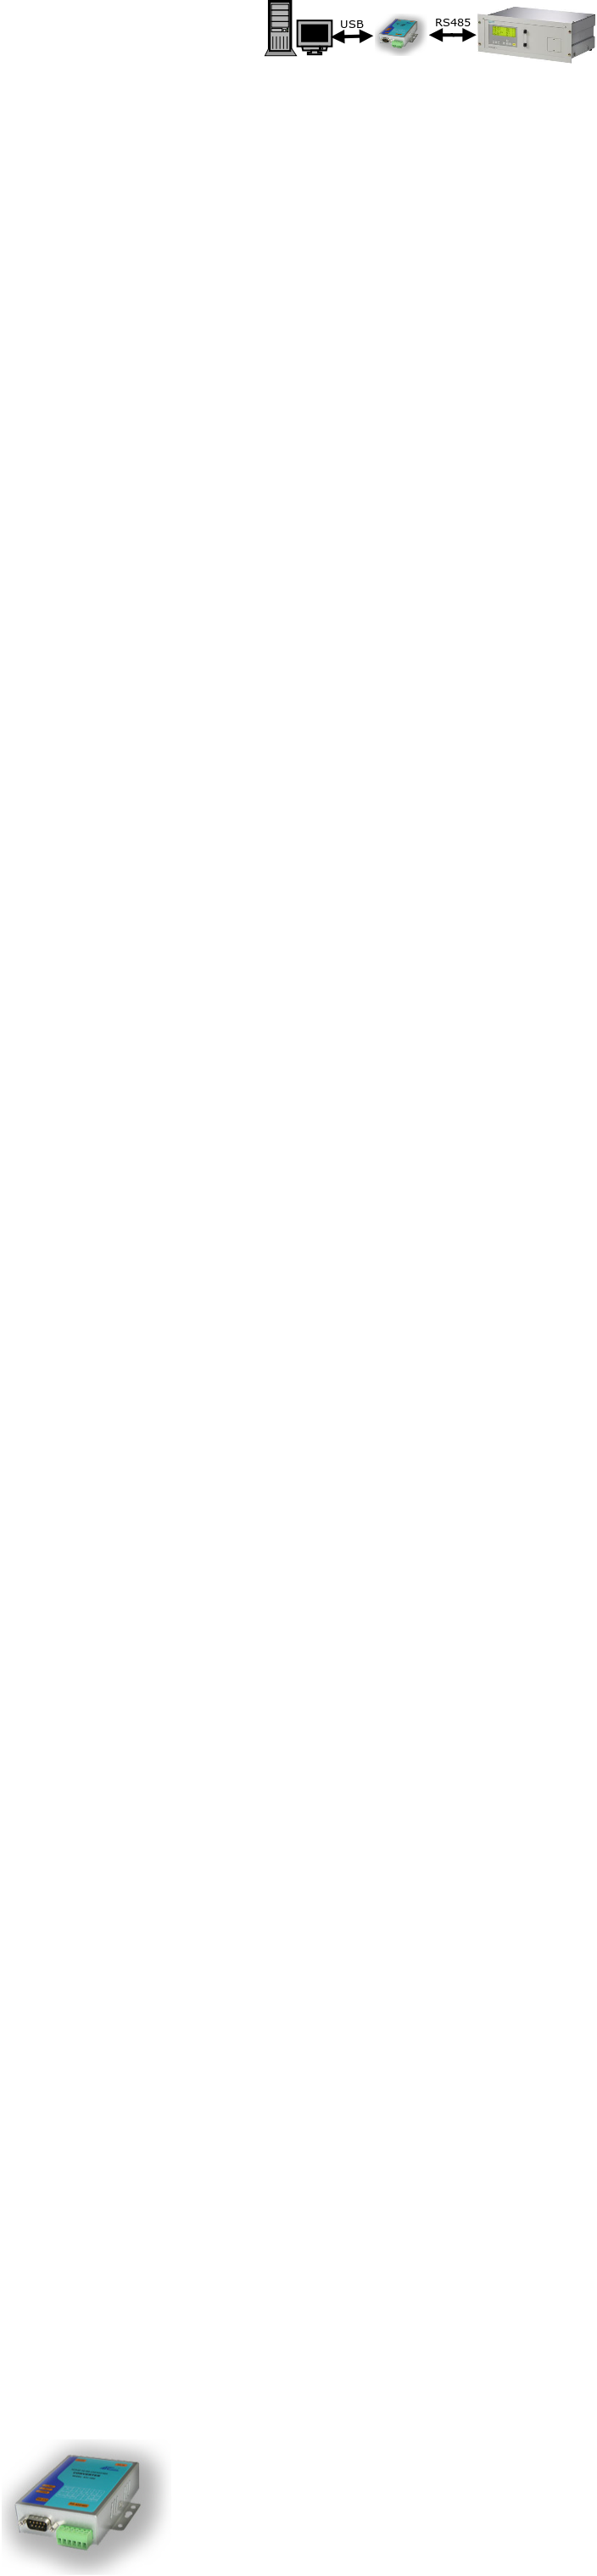
\includegraphics[width=0.8\textwidth]{images/schemat1} 	\caption{Schemat stanowiska prototypowego} \label{schemat1} \end{figure} 
Na~potrzeby realizacji projektu stworzono stanowisko laboratoryjne, którego schemat przedstawia Rysunek~\ref{schemat1}. Składa się ono~z:
\begin{itemize}
\item Komputera,
\item Konwertera ATC-850,
\item ULTRAMAT 23.
\end{itemize}
\indent
\indent Komputery na, których powstała wersja rozwojowa projekty pracowały na systemach operacyjnych Linux Ubuntu w~wersji 32 oraz 64~bitowej. Do~połączenia komputera z~urządzeniem ULTRAMAT~23 zastosowano izolowany konwerter~USB do~RS-232/422/485, moduł ATC-850 jest automatycznie wykrywany i~instalowany jako standardowy port~COM. Stosowane w~tej fazie projektu urządzenie pomiarowe potrafiło mierzyć zawartość $ CO_2 $, $ CO $, $ O_2 $ oraz $ NO_2 $ ??

\subsubsection{Stanowisko docelowe}
\begin{figure}[!htb] 	\centering 	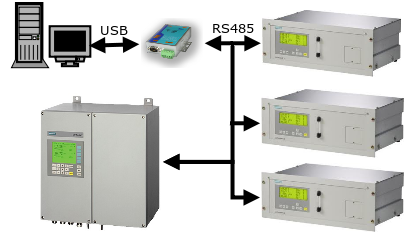
\includegraphics[width=0.8\textwidth]{images/schemat2} 	\caption{Schemat stanowiska docelowego} \label{schemat2} \end{figure} 
Docelowo zrealizowany projekt ma być uruchamiany na~stanowisku, którego schemat przedstawia Rysunek~\ref{schemat2}. Składa się ono~z:
\begin{itemize}
\item Komputera,
\item Konwertera ATC-850,
\item 3x ULTRAMAT 23,
\item ULTRAMAT 6.
\end{itemize}
\indent
\indent Stanowisko docelowe różni się od stanowiska prototypowego po pierwsze systemem operacyjnym, który pracuje na komputerze i jest to Windows XP. Po drugie stanowisko docelowe posiada więcej urządzeń pomiarowych, a jest ich dokładnie cztery i mierzą wartości przedstawione w Tabeli~\ref{tab:docelowe}.

\begin{table}[h]
\centering
\begin{tabular}{|l|l|}
\hline Urządzenie & Wielkości mierzone \\ 
\hline ULTRAMAT~6 & $ NH_3 [vpm] $ \\ 
\hline ULTRAMAT~23 & $ CH_4 [\%], CO [\%], CO_2 [\%], O_2 [\%] $ \\ 
\hline ULTRAMAT~23 & $  $ \\ 
\hline ULTRAMAT~23 & $  $ \\ 
\hline 
\end{tabular} 
\caption{Urządzenia docelowe wraz z wartościami mierzonymi}
\label{tab:docelowe}
\end{table}

\subsection{Analiza tematu}
Analiza tematu polegała przede wszystkim na zapoznaniu się z~narzędziami programistycznymi do~tworzenia oprogramowania sterownika oraz wizualizacji.
Poznanie tych podstaw pozwoliło dobrać język odpowiedni do~realizacji poszczególnych zadań.

\subsection{Założenia}
%Stworzone oprogramowanie dla Robota Fishertechnik ma działać na sterownikach firmy Siemens oraz ma zostać stworzone przy użyciu środowiska Step 7. Funkcjonalności robota, jakie mają wchodzić w~skład projektu, to:
Oprogramowanie do zbierania danych pomiarowych powinno zostać stworzone przy użyciu technologii pozwalającej działać na~różnych systemach operacyjnych bez~skomplikowanych zabiegów.Funkcjonalności wchodzące w~skład projektu,~to:
\begin{itemize}
\item sterowanie ręczne z~pilota podłączonego bezpośrednio do~sterownika,
\item sterowanie ręczne z~wizualizacji,
\item sterowanie automatyczne, 
\item wizualizacja bieżących pomiarów,
\item generowanie raportu z pomiaru jako plik arkusza kalkulacyjnego,
\item generowanie raportu z pomiaru jako plik do wydruku z wynikami np. format~PDF,
\item .
\end{itemize}
\indent
\indent Powyżej zostały wymienione założenia podstawowe, jednak autorzy nie~wykluczają zrealizowania dodatkowych zadań, które nie~zostały zamieszczone w~pierwotnej koncepcji realizacji projektu.

\subsection{Plan pracy}
Realizacja projektu została podzielona na następujące etapy:
\begin{itemize}
\item Przygotowanie stanowiska, zebranie odpowiednich materiałów i~literatury,
\item Analiza wymagań funkcjonalnych aplikacji,
\item Projektowanie struktury oprogramowania i~interfejsów wymiany danych,
\item Implementacja,
\item Testowanie i~uruchamianie,
\item Przedstawienie projektu i~ewentualne korekty.
\end{itemize}
\indent
\indent Powyższy plan pracy stanowił dla autorów wyznacznik kolejnych działań. Jednak powszechnie wiadomo, że w~praktyce poszczególne punkty są~wymienne i~wpływają na siebie wzajemnie.

\begin{table}[h]
\centering
\begin{tabular}{|p{0.15\textwidth}|p{0.15\textwidth}|p{0.7\textwidth}|}
\hline \textbf{Termin} & \textbf{Osoba} & \textbf{Zadanie} \\ 
\hline\hline 11.03 -- 17.03 & Wszyscy & Wybór tematu. \\ 
\hline 18.03 -- 20.03 & Wszyscy & Określenie celu i~zakresu, przygotowanie harmonogramu, podział zadań. \\ 
\hline 21.03 & Wszyscy & Analiza sprzętu oraz dokumentacji. \\ 
\hline 22.03 -- 23.03 & Wszyscy & Analiza oraz porównanie dopuszczalnych rozwiązań z wykorzystaniem protokołu ELAN lub~Profibus. \\ 
\hline 24.03 -- 25.03 & Wszyscy & Analiza wybranego protokołu oraz potrzebnego sprzętu do połączenia z komputerem (np. konwerter RS-485 $\Leftrightarrow\Leftrightarrow$ USB ). \\ 
\hline 25.03 -- 02.04 & Wszyscy & Implementacja wybranych fragmentów protokołu. \\ 
\hline 29.03 -- 17.04 & Damian & Przygotowanie podstawowej wersji interfejsu użytkownika, umożliwiającej przetestowanie implementacji protokołu. \\ 
\hline 03.04 -- 18.04 & Grzegorz & Rozwinięcie podstawowej wersji protokołu – interpretacja i~przetwarzanie odbieranych danych. \\ 
\hline 20.04 -- 01.05 & Grzegorz & Stworzenie modelu bazy danych i~połączenia ORM. \\ 
\hline 19.04 -- 05.05 & Damian & Wykrycie i wizualizacja struktury sieci oraz odbieranych danych. \\ 
\hline 03.05 -- 06.05 & Damian & Generowanie PDF. \\ 
\hline 04.05 -- 10.05 & Grzegorz  & Generowanie XLS. \\ 
\hline 13.05 -- 22.05 & Grzegorz & Zarządzanie ustawieniami urządzeń. \\ 
\hline 27.05 -- 05.06 & Damian & Poprawki w GUI. \\ 
\hline 01.06 -- 08.06 & Wszyscy & Instrukcja użytkownika oraz dokumentacja. \\ 
\hline 
\end{tabular} 
\caption{Szczegółowy plan pracy wraz z~harmonogramem i~osobami odpowiedzialnymi}
\label{tab:harmonogram}
\end{table}